% How a velocity field transforms under a change of coordinates Phi.
%
% A velocity field v assigns a vector to each point; a curve gamma through
% x with gamma-dot(0) = v(x) realizes that vector as an actual velocity. Push
% the curve through Phi and differentiate at t=0: the new tangent is
% J(x) v(x) = v'(x'). That is the whole content -- the field transforms the way
% a TANGENT VECTOR does, because it IS one, and the operator that carries it is
% the JACOBIAN of Phi, not Phi.
%
% Notation tracks the "Why the Jacobian shows up" derivation in
% src/content/journal/notes/symmetry-transformations.mdx -- plain gamma(t) for
% the curve, Phi(gamma(t)) for its image, J(x) for the derivative. Keep them in
% step if that derivation is reworded.
%
% THE ONE THING THAT MUST BE GEOMETRICALLY EXACT: gamma is tangent to the field
% at x, and Phi(gamma) is tangent to the transformed field at x'. Everything
% here is built so that tangency is exact rather than eyeballed:
%
%   left  -- streamlines are concentric circular arcs about C=(\CxL,\CyL). The
%            tangent to such an arc at polar angle phi is exactly phi-270 deg.
%            gamma is two `to[out=,in=]' segments meeting at x, BOTH using that
%            angle, so gamma and the arc share a tangent line at x to the pixel.
%   right -- streamlines are straight at \thR; gamma' meets x' with out=\thR and
%            in=\thR+180. Same trick, same exactness.
%
% gamma deliberately curves the OPPOSITE way from the streamline it touches, so
% it kisses that streamline at x and peels away on both sides (visible tangency)
% while crossing the neighbouring streamlines transversally -- gamma is any curve
% with the right velocity at t=0, not an integral curve of the field.
%
% See _template.tex / _preamble.tex for the shared setup.
\ifnum\pdfoutput>0
\documentclass[tikz,border=3pt]{standalone}         % pdflatex → PDF proof
\else
\documentclass[tikz,border=3pt,dvisvgm]{standalone} % latex   → web SVG
\fi
% Shared setup for all site figures — \input by every figures/*.tex.
% Change the palette, font size, or driver logic HERE and every figure inherits
% it on next rebuild. See src/assets/blog/README.md for the full workflow.
%
% NOTE: this file is \input AFTER \documentclass (it needs amsmath/tikz loaded),
% but the \documentclass line itself carries the driver switch and must stay in
% each figure — see _template.tex. Keep figure .tex files starting from that
% template so the driver logic is never forgotten.

\usepackage{amsmath}

% --- Palette: sentinel hexes = the LIGHT-theme values from DESIGN.md. ----------
% The PDF proof / Overleaf output therefore look like the light rendering, and
% fig.sh rewrites each hex to its themed CSS variable in the web SVG:
%   ink    #000000 -> var(--color-text-main, currentColor)   (also all black strokes)
%   accent #003366 -> var(--color-accent, #003366)
%   muted  #555555 -> var(--color-text-muted, #555555)
%   figred #b91c1c -> var(--fig-red, #b91c1c)
%   figblue   #1d4ed8 -> var(--fig-blue, #1d4ed8)
%   figorange #c2410c -> var(--fig-orange, #c2410c)
\definecolor{ink}{HTML}{000000}
\definecolor{accent}{HTML}{003366}
\definecolor{muted}{HTML}{555555}
\definecolor{figred}{HTML}{B91C1C}
\definecolor{figblue}{HTML}{1D4ED8}
\definecolor{figorange}{HTML}{C2410C}

% --- Figure body font size = site body text. ---------------------------------
% The site renders body text at 18px ≈ 13.5pt. dvisvgm emits the SVG at its
% intrinsic point size and <Figure> shows it ~1:1, so to make figure labels match
% surrounding prose we set the figure's \normalsize to 13.5/16pt. Individual
% labels can still deviate with font=\small / font=\large as needed. Computer
% Modern matches the KaTeX body math, so $dg_p(v)$ reads identically in both.
\newcommand{\figfontsize}{\fontsize{13.5}{16}\selectfont}

% Apply it as the default font for every tikzpicture, plus sane global defaults.
% Dimension figures in mm (x=1mm,y=1mm) so geometry and this pt-based text stay
% independent — scale the drawing by editing coordinates, not the type size.
\tikzset{
  every picture/.style = {font=\figfontsize, line join=round},
  edge/.style          = {line width=1pt},
  hair/.style          = {line width=1pt},
}

% arrows.meta -> Stealth tips; decorations.markings -> flow arrowheads placed
% partway ALONG a streamline (an end-anchored `->' would tip only the last one).
\usetikzlibrary{arrows.meta, decorations.markings}

\begin{document}
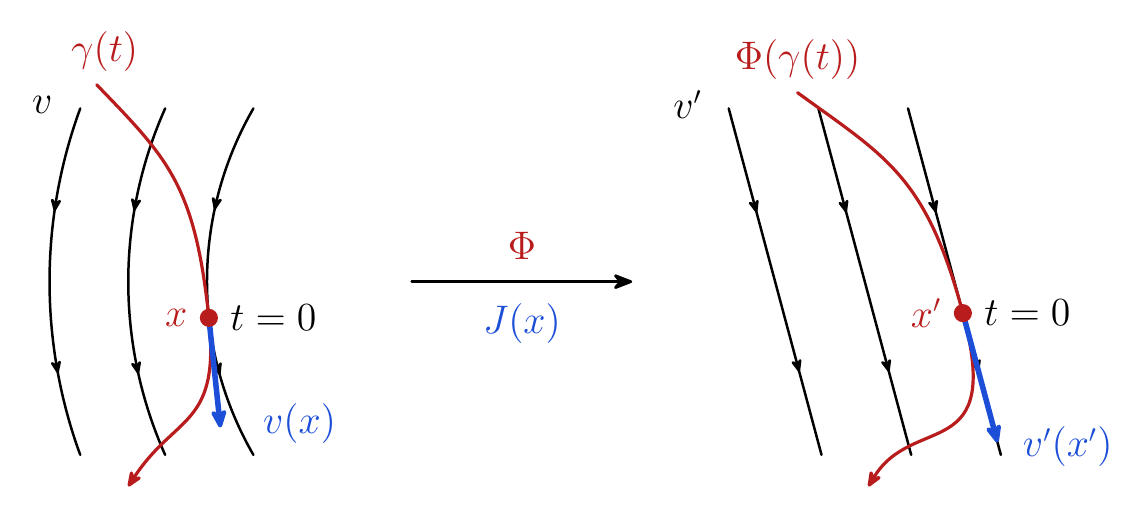
\begin{tikzpicture}[x=1mm, y=1mm]

  % --- Shared styles ----------------------------------------------------------
  % Streamlines are context: thinner than the palette default so the tangent
  % vector, which necessarily lies ON one of them, still reads as the subject.
  \tikzset{
    stream/.style = {line width=0.9pt, ink, line cap=round,
      postaction={decorate},
      decoration={markings,
        mark=at position 0.30 with {\arrow{Stealth[length=2.1mm, width=1.7mm, round]}},
        mark=at position 0.76 with {\arrow{Stealth[length=2.1mm, width=1.7mm, round]}}}},
    curve/.style  = {line width=1.15pt, figred, line cap=round,
      -{Stealth[length=2.6mm, width=2.1mm, round]}},
    % The tangent vector is the point of the figure and it sits on top of a
    % streamline (that is what tangency MEANS), so it has to win on weight.
    tvec/.style   = {line width=2pt, figblue, line cap=round,
      -{Stealth[length=3.1mm, width=2.6mm, round]}},
    dot/.style    = {figred},
    lbl/.style    = {inner sep=1.6pt},
  }

  % Both panels span the same band of y so the two fields read as the same
  % region of space seen in two coordinate systems.
  \def\ytop{50}\def\ybot{6}

  % ===========================================================================
  % LEFT PANEL -- curved field v
  % ===========================================================================
  % Streamlines: concentric arcs about C, drawn over the y-band [\ybot,\ytop].
  % For radius r that band is the polar half-angle asin(\yhalf/r) either side of
  % 180 deg, so every arc starts and ends at the same height.
  \def\CxL{72}\def\CyL{28}          % arc center, off to the right
  \def\yhalf{22}                    % half the y-band: \CyL +- \yhalf
  \def\rin{44}                      % radius of the arc that gamma touches

  \foreach \r in {44, 54, 64}{
    \pgfmathsetmacro{\D}{asin(\yhalf/\r)}
    \draw[stream]
      ({\CxL + \r*cos(180-\D)}, {\CyL + \r*sin(180-\D)})
      arc[start angle={180-\D}, end angle={180+\D}, radius=\r];
  }

  % The base point x, on the innermost (rightmost) arc. Putting it there leaves
  % the whole right half of the panel free for gamma and the labels.
  \def\phix{186}                                   % polar angle of x about C
  \pgfmathsetmacro{\xax}{\CxL + \rin*cos(\phix)}   % 28.241
  \pgfmathsetmacro{\xay}{\CyL + \rin*sin(\phix)}   % 23.401
  % Tangent to a circle traversed with INCREASING phi is exactly phi-270 deg.
  % This single number is what makes the figure honest: the arc, gamma and the
  % velocity arrow all leave x along it.
  \pgfmathsetmacro{\tanL}{\phix - 270}             % -84
  \pgfmathsetmacro{\inL}{\tanL + 180}              % 96 (arrive moving at \tanL)

  % gamma: crosses the outer streamlines, kisses the inner one at x. Its
  % curvature there is opposite to the arc's, so the two separate on both sides
  % of x instead of merging into one indistinguishable stroke.
  %
  % EXPLICIT control points, not `to[out=,in=]'. Both express the same tangent
  % angle, but `to' places its controls close to the endpoints, so the curve runs
  % along its CHORD and only swings onto the stated angle in the last fraction of
  % a mm. The exit angle is then technically right and visibly wrong: rendered,
  % gamma cornered straight through the streamline. Naming the control distances
  % (17mm in, 14mm out) makes gamma hug the tangent line for a real distance, so
  % the contact reads as tangency. Measured on the render: gamma and the arc are
  % 0.7mm apart 5-7mm either side of x (a kiss) and 3-4mm apart by 10-15mm out.
  \draw[curve] (14,53)
    .. controls +(-46:13) and +({\inL}:17) .. ({\xax},{\xay})
    .. controls +({\tanL}:14) and +(57:11) .. (18,2);

  % The velocity vector at t=0, along the tangent line.
  \def\vlenL{14}
  \pgfmathsetmacro{\tipLx}{\xax + \vlenL*cos(\tanL)}
  \pgfmathsetmacro{\tipLy}{\xay + \vlenL*sin(\tanL)}
  \draw[tvec] ({\xax},{\xay}) -- ({\tipLx},{\tipLy});
  \fill[dot] ({\xax},{\xay}) circle[radius=1.15];

  % Labels. \bs{v} sits just off the top end of the outermost arc, so it reads as
  % naming the bundle rather than floating in the margin.
  \node[lbl, text=ink,     anchor=east]  at (9,50.5)          {$\bs{v}$};
  \node[lbl, text=figred,  anchor=south] at (15,54)           {$\gamma(t)$};
  \node[lbl, text=figred,  anchor=east]  at ({\xax-2.1},{\xay})  {$\bs{x}$};
  \node[lbl, text=ink,     anchor=west]  at ({\xax+2.1},{\xay})  {$t=0$};
  % Just the vector, not "gamma-dot(0) = v(x)": the paragraph this figure sits
  % under already states that identity, and the figure's own job is the geometry.
  \node[lbl, text=figblue, anchor=west]  at (34.5,10)         {$\bs{v}(\bs{x})$};

  % ===========================================================================
  % THE MAP -- Phi moves points and curves, its Jacobian J(x) moves tangent
  % vectors. Colouring each label after the object it acts on is the link
  % between the panels, and the split IS the derivation's punchline: the two
  % labels sit on one arrow because they are two actions of one transformation.
  % ===========================================================================
  \draw[edge, ink, line cap=round, -{Stealth[length=3mm, width=2.3mm, round]}]
    (54,28) -- (82,28);
  \node[lbl, text=figred,  anchor=south] at (68,30.2) {$\Phi$};
  \node[lbl, text=figblue, anchor=north] at (68,25.8) {$J(\bs{x})$};

  % ===========================================================================
  % RIGHT PANEL -- straightened field v'
  % ===========================================================================
  \begin{scope}[shift={(86,0)}]
    \def\thR{-75}                      % streamline direction (and so v')
    \def\xbx{38}\def\xby{24}           % x' sits on the rightmost line
    \def\sep{11}                       % perpendicular spacing between lines
    \pgfmathsetmacro{\inR}{\thR + 180} % 105 (arrive moving at \thR)
    % cot of the line direction: how far x moves per unit y along a streamline.
    \pgfmathsetmacro{\ct}{cos(\thR)/sin(\thR)}

    % Three parallel lines, offset along the normal from x''s line and clipped to
    % the same y-band as the arcs opposite. The normal is \thR-90, NOT \thR+90:
    % the sibling lines have to fall to the LEFT of x', mirroring the left panel
    % where x sits on the innermost (rightmost) arc. With +90 they land on the
    % other side and x' ends up on the leftmost line, with the labels then having
    % to jump the whole bundle.
    \foreach \k in {0,1,2}{
      \pgfmathsetmacro{\Px}{\xbx + \k*\sep*cos(\thR-90)}
      \pgfmathsetmacro{\Py}{\xby + \k*\sep*sin(\thR-90)}
      \draw[stream]
        ({\Px + (\ytop-\Py)*\ct}, \ytop) -- ({\Px + (\ybot-\Py)*\ct}, \ybot);
    }

    % Phi(gamma): the image curve. Same story as gamma -- transversal to the
    % field in general, tangent to it at x' -- but distorted, since Phi is not
    % linear. Explicit control distances again, for the reason given on gamma --
    % and the departing one runs LONGER here (20mm vs 14mm opposite). Over there
    % the streamline is an arc bending away from the contact on its own, so half
    % the visible separation is the field's doing; here the streamline is dead
    % straight and every bit of it has to come from this curve, which at 16mm
    % rendered as a corner at x'. 20mm puts its radius of curvature near 64mm:
    % 0.6mm off the line 7mm out (a kiss), 3mm off by 12mm out.
    \draw[curve] (17,52)
      .. controls +(-36:14) and +({\inR}:18) .. ({\xbx},{\xby})
      .. controls +({\thR}:20) and +(59:11) .. (26,2);

    % The transformed velocity. Longer than v(x): dPhi_x stretches as well as
    % turns, so drawing the two arrows the same length would be a quiet lie.
    \def\vlenR{17}
    \pgfmathsetmacro{\tipRx}{\xbx + \vlenR*cos(\thR)}
    \pgfmathsetmacro{\tipRy}{\xby + \vlenR*sin(\thR)}
    \draw[tvec] ({\xbx},{\xby}) -- ({\tipRx},{\tipRy});
    \fill[dot] ({\xbx},{\xby}) circle[radius=1.15];

    % Labels
    \node[lbl, text=ink,     anchor=east]  at (5.5,50.5)          {$\bs{v}'$};
    \node[lbl, text=figred,  anchor=south] at (17,53)             {$\Phi(\gamma(t))$};
    \node[lbl, text=figred,  anchor=east]  at ({\xbx-2.1},{\xby}) {$\bs{x}'$};
    \node[lbl, text=ink,     anchor=west]  at ({\xbx+2.1},{\xby}) {$t=0$};
    \node[lbl, text=figblue, anchor=west]  at (45,7)              {$\bs{v}'(\bs{x}')$};
  \end{scope}
\end{tikzpicture}
\end{document}
